\documentclass{standalone}
\usepackage{ tikz }
\usepackage{ xparse }
\usepackage{../../../macros}

\begin{document}
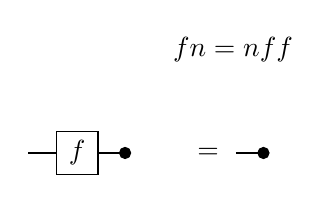
\begin{tikzpicture}[yscale=-1,x=1em,y=1.25em]

    \draw (0.5,0) -- (1.5,0);
    \node[draw, minimum height = 1.5em, minimum width = 1.5em, anchor = west] at (1.5,0){$f$};
    \draw (3,0) -- (4,0);
    \filldraw (4,0) circle (2pt);

    \node at (7,0) {$=$};
    \node at (7.9,-3) {$f \seq \ccopy{n} = \ccopy{n} \seq f \tensor f$};

    \draw (8,0) -- (9,0);
    \filldraw (9,0) circle (2pt);
\end{tikzpicture}
\end{document}